\documentclass[a4paper,12pt]{article}

% --- Tiếng Việt + mã UTF-8 ---
\usepackage[utf8]{inputenc}
\usepackage[T5]{fontenc}
\usepackage[vietnamese]{babel}

% --- Bố cục trang ---
\usepackage{geometry}
\geometry{top=2.5cm, bottom=2.5cm, left=3cm, right=2cm}

% --- Toán ---
\usepackage{amsmath}
\usepackage{amssymb}

% --- Hình ảnh ---
\usepackage{graphicx}
\graphicspath{{img/}}

% --- Liên kết ---
\usepackage{hyperref}

\begin{document}

% ================= TRANG BÌA =================
\begin{center}
ỦY BAN NHÂN DÂN THÀNH PHỐ HỒ CHÍ MINH

TRƯỜNG ĐẠI HỌC SÀI GÒN

KHOA TOÁN -- ỨNG DỤNG


\includegraphics[width=4cm]{SGU-LOGO.png}

\textbf{BÀI TẬP 4: MẠNG MLP}

Môn: Học sâu (Deep Learning)

Họ và tên: Đinh Quang Minh

MSSV: 3123580024

Lớp: DDU1231

Ngành: Khoa học dữ liệu

Giảng viên hướng dẫn: TS. Đỗ Như Tài

Học kỳ I, năm học 2026

TP. Hồ Chí Minh, tháng 10 năm 2026
\end{center}

\newpage

% ================================================================
\section*{Bài 1. Lan truyền xuôi và cập nhật trọng số của một nơ-ron}

Mạng gồm hai đầu vào $x_1, x_2$, một nút bias $b$ và một nơ-ron đầu ra dùng sigmoid.
Trọng số ban đầu $w_1 = w_2 = w_{bias} = 0.25$; dữ liệu $x_1 = 0.1$, $x_2 = 0.2$, $b = 1$;
đầu ra mong đợi $y = 1$; tốc độ học $\alpha = 0.1$.

\begin{center}
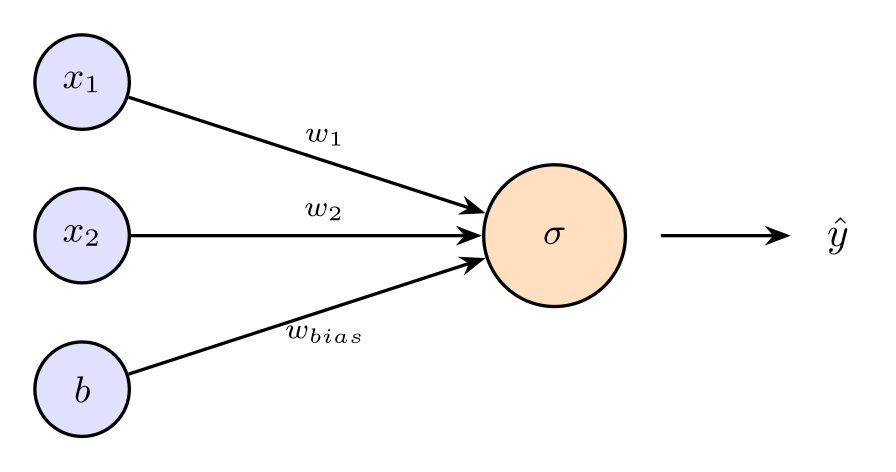
\includegraphics[width=0.62\textwidth]{b1_net.png}
\end{center}

\textbf{1. Tổng có trọng số.}
\[ z = w_1x_1 + w_2x_2 + w_{bias}b
     = 0.25\cdot 0.1 + 0.25\cdot 0.2 + 0.25\cdot 1 = 0.325. \]

\textbf{2. Đầu ra dự đoán.}
\[ \hat{y} = \sigma(z) = \frac{1}{1+e^{-0.325}} \approx 0.580542. \]

\textbf{3. Hàm mất mát.} Vì $y = 1$ nên số hạng $(1-y)\ln(1-\hat{y})$ bằng 0:
\[ L = -\bigl[y\ln\hat{y} + (1-y)\ln(1-\hat{y})\bigr]
     = -\ln(0.580542) \approx 0.543793. \]

\textbf{4. Đạo hàm theo quy tắc dây chuyền.} Trước hết
\[ \frac{\partial L}{\partial \hat{y}} = -\frac{y}{\hat{y}} + \frac{1-y}{1-\hat{y}}
   = -\frac{1}{0.580542} \approx -1.722527, \]
và với sigmoid thì $\sigma'(z) = \hat{y}(1-\hat{y}) = 0.580542\cdot 0.419458 \approx 0.243513$, nên
\[ \frac{\partial L}{\partial z}
   = \frac{\partial L}{\partial \hat{y}}\cdot\frac{\partial \hat{y}}{\partial z}
   \approx -1.722527\cdot 0.243513 \approx -0.419458. \]
Kết quả này đúng bằng $\hat{y} - y$, phù hợp với công thức quen thuộc của BCE kết hợp sigmoid.
Vì $z = w_1x_1 + w_2x_2 + w_{bias}b$ nên
\[ \frac{\partial z}{\partial w_1} = x_1,\qquad
   \frac{\partial z}{\partial w_2} = x_2,\qquad
   \frac{\partial z}{\partial w_{bias}} = b, \]
suy ra
\[ \frac{\partial L}{\partial w_1} = -0.419458\cdot 0.1 \approx -0.0419458, \]
\[ \frac{\partial L}{\partial w_2} = -0.419458\cdot 0.2 \approx -0.0838915, \]
\[ \frac{\partial L}{\partial w_{bias}} = -0.419458\cdot 1 \approx -0.4194577. \]

\textbf{5. Cập nhật trọng số.} Áp dụng $w \leftarrow w - \alpha\dfrac{\partial L}{\partial w}$:
\[ w_1 = 0.25 - 0.1\cdot(-0.0419458) \approx 0.2541946, \]
\[ w_2 = 0.25 - 0.1\cdot(-0.0838915) \approx 0.2583892, \]
\[ w_{bias} = 0.25 - 0.1\cdot(-0.4194577) \approx 0.2919458. \]

\textbf{6. Tính lại sau một lần cập nhật.}
\[ z' = 0.2541946\cdot 0.1 + 0.2583892\cdot 0.2 + 0.2919458\cdot 1 \approx 0.369043, \]
\[ \hat{y}' = \sigma(0.369043) \approx 0.591228, \]
\[ L' = -\ln(0.591228) \approx 0.525554. \]
Hàm mất mát giảm từ $0.543793$ xuống $0.525554$ (giảm $0.018239$). Đầu ra dự đoán tăng từ
$0.5805$ lên $0.5912$, tức đã tiến gần giá trị mong đợi $y=1$ hơn, nên bước cập nhật đi đúng
hướng.

% ================================================================
\section*{Bài 2. Biểu diễn mạng nơ-ron bằng vector và ma trận}

Mạng có hai đầu vào $x_1, x_2$, một nút bias $b$ và hai nơ-ron đầu ra. Mọi trọng số và trọng
số bias đều bằng $0.5$; $x_1 = 0.1$, $x_2 = 0.2$, $b = 1$; đầu ra mong đợi
$\mathbf{y} = [0,\ 1]^T$. Theo gợi ý của đề, em giả định cả hai nơ-ron đầu ra dùng sigmoid.

\begin{center}
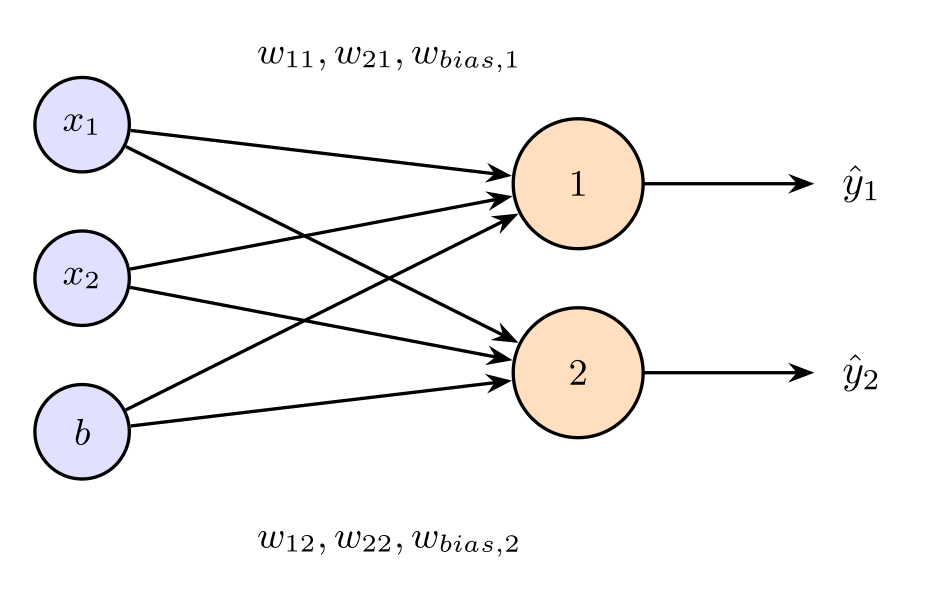
\includegraphics[width=0.72\textwidth]{b23_net.png}
\end{center}

\textbf{1. Vector đầu vào, ma trận trọng số, vector bias.}
\[ \mathbf{x} = \begin{bmatrix} x_1 \\ x_2 \end{bmatrix} = \begin{bmatrix} 0.1 \\ 0.2 \end{bmatrix},
   \qquad
   W = \begin{bmatrix} w_{11} & w_{21} \\ w_{12} & w_{22} \end{bmatrix}
     = \begin{bmatrix} 0.5 & 0.5 \\ 0.5 & 0.5 \end{bmatrix},
   \qquad
   \mathbf{b} = \begin{bmatrix} 0.5 \\ 0.5 \end{bmatrix}, \]
trong đó hàng của $W$ ứng với từng nơ-ron đầu ra, cột ứng với từng đầu vào.

\textbf{2. Phương trình lan truyền xuôi dạng vector.}
\[ \mathbf{z} = W\mathbf{x} + \mathbf{b}\,b, \qquad
   \hat{\mathbf{y}} = f(\mathbf{z}), \]
trong đó $\mathbf{b}$ là vector bias còn $b = 1$ là đầu vào bias.

\textbf{3. Vector tổng có trọng số.}
\[ z_1 = 0.5\cdot 0.1 + 0.5\cdot 0.2 + 0.5\cdot 1 = 0.65, \]
\[ z_2 = 0.5\cdot 0.1 + 0.5\cdot 0.2 + 0.5\cdot 1 = 0.65, \]
nên $\mathbf{z} = [0.65,\ 0.65]^T$.

\textbf{4. Vector đầu ra.} Với $f$ là sigmoid áp dụng cho từng phần tử:
\[ \hat{\mathbf{y}} = f(\mathbf{z})
   = \begin{bmatrix} \sigma(0.65) \\ \sigma(0.65) \end{bmatrix}
   \approx \begin{bmatrix} 0.657010 \\ 0.657010 \end{bmatrix}. \]

\textbf{5. Tính bằng phương pháp vectorized.}
\[
W\mathbf{x} = \begin{bmatrix} 0.5 & 0.5 \\ 0.5 & 0.5 \end{bmatrix}
             \begin{bmatrix} 0.1 \\ 0.2 \end{bmatrix}
           = \begin{bmatrix} 0.05 + 0.10 \\ 0.05 + 0.10 \end{bmatrix}
           = \begin{bmatrix} 0.15 \\ 0.15 \end{bmatrix},
\]
\[
\mathbf{z} = \begin{bmatrix} 0.15 \\ 0.15 \end{bmatrix}
           + \begin{bmatrix} 0.5 \\ 0.5 \end{bmatrix}\cdot 1
           = \begin{bmatrix} 0.65 \\ 0.65 \end{bmatrix}.
\]
Kết quả trùng với cách tính từng nơ-ron ở trên.

\textbf{6. So sánh và lợi ích của vectorization.} Tính từng nơ-ron phải viết hai lần cùng một
biểu thức (mỗi lần ba phép nhân và hai phép cộng); cách ma trận chỉ cần một phép nhân
$W\mathbf{x}$ là ra cả hai nơ-ron. Khi số nơ-ron tăng, cách ma trận còn tận dụng được thư viện
tối ưu và GPU nên chạy nhanh hơn nhiều, code cũng ngắn và ít lỗi hơn.

% ================================================================
\section*{Bài 3. Lan truyền ngược với các hàm kích hoạt khác nhau}

Kiến trúc giống Bài 2: hai nơ-ron đầu ra, mọi trọng số và bias bằng $0.5$,
$x_1 = 0.1$, $x_2 = 0.2$, $b = 1$, đầu ra mong đợi $y_1 = 0$, $y_2 = 1$, $\alpha = 0.1$.

\textbf{Lưu ý về hàm mất mát.} Đầu ra của tanh nằm trong $(-1,1)$ còn ReLU có thể nhận giá trị
bất kỳ, nên không thể áp dụng trực tiếp Binary Cross-Entropy. Vì vậy em dùng
\textbf{MSE} cho nơ-ron 1 và \textbf{BCE} cho nơ-ron 2 (nơ-ron này dùng sigmoid nên đầu ra là
xác suất):
\[ L = L_1 + L_2 = \frac{1}{2}(\hat{y}_1 - y_1)^2
   - \bigl[y_2\ln\hat{y}_2 + (1-y_2)\ln(1-\hat{y}_2)\bigr]. \]

\subsection*{Trường hợp 1: $f_1 = \tanh$, $f_2 = \sigma$}

\textbf{1. Tổng có trọng số.} Vì các trọng số đều bằng $0.5$ nên giống Bài 2:
\[ z_1 = 0.5x_1 + 0.5x_2 + 0.5b = 0.65, \qquad z_2 = 0.65. \]

\textbf{2. Đầu ra của mạng.}
\[ \hat{y}_1 = \tanh(0.65) \approx 0.571670, \qquad
   \hat{y}_2 = \sigma(0.65) \approx 0.657010. \]

\textbf{3. Hàm mất mát.}
\[ L_1 = \frac{1}{2}(\hat{y}_1 - y_1)^2 = \frac{1}{2}(0.571670)^2 \approx 0.163403, \]
\[ L_2 = -\ln(\hat{y}_2) = -\ln(0.657010) \approx 0.420055, \]
\[ L = L_1 + L_2 \approx 0.583459. \]

\textbf{4. Gradient theo quy tắc dây chuyền.}
Với nơ-ron 1:
\[ \frac{\partial L_1}{\partial \hat{y}_1} = \hat{y}_1 - y_1 = 0.571670, \qquad
   f_1'(z_1) = 1 - \tanh^2(z_1) = 1 - 0.326806 = 0.673194, \]
\[ \frac{\partial L}{\partial z_1} = 0.571670\cdot 0.673194 \approx 0.384844. \]
Với nơ-ron 2 (BCE kết hợp sigmoid):
\[ \frac{\partial L}{\partial z_2} = \hat{y}_2 - y_2 = 0.657010 - 1 = -0.342990. \]
Từ $\partial z_j/\partial w_{ij} = x_i$ và $\partial z_j/\partial w_{bias,j} = b$:
\[ \frac{\partial L}{\partial w_{11}} = 0.384844\cdot 0.1 \approx 0.0384844, \quad
   \frac{\partial L}{\partial w_{21}} = 0.384844\cdot 0.2 \approx 0.0769689, \]
\[ \frac{\partial L}{\partial w_{bias,1}} = 0.384844\cdot 1 \approx 0.3848445, \]
\[ \frac{\partial L}{\partial w_{12}} = -0.342990\cdot 0.1 \approx -0.0342990, \quad
   \frac{\partial L}{\partial w_{22}} = -0.342990\cdot 0.2 \approx -0.0685979, \]
\[ \frac{\partial L}{\partial w_{bias,2}} \approx -0.3429895. \]

\textbf{5. Cập nhật trọng số.}
\[ w_{11} \approx 0.496152, \quad w_{21} \approx 0.492303, \quad w_{bias,1} \approx 0.461516, \]
\[ w_{12} \approx 0.503430, \quad w_{22} \approx 0.506860, \quad w_{bias,2} \approx 0.534299. \]

\textbf{6. Kết quả sau cập nhật.}
\[ z_1' \approx 0.609591, \qquad z_2' \approx 0.686014, \]
\[ \hat{y}_1' = \tanh(0.609591) \approx 0.543839, \qquad
   \hat{y}_2' = \sigma(0.686014) \approx 0.665080, \]
\[ L' \approx 0.555729 \quad (\text{giảm } 0.027730 \text{ so với } 0.583459). \]

\subsection*{Trường hợp 2: $f_1 = \mathrm{ReLU}$, $f_2 = \sigma$}

\textbf{1. Tổng có trọng số.} Vẫn là $z_1 = z_2 = 0.65$.

\textbf{2. Đầu ra của mạng.}
\[ \hat{y}_1 = \mathrm{ReLU}(0.65) = 0.65, \qquad
   \hat{y}_2 = \sigma(0.65) \approx 0.657010. \]

\textbf{3. Hàm mất mát.}
\[ L_1 = \frac{1}{2}(0.65)^2 \approx 0.211250, \qquad
   L_2 = -\ln(0.657010) \approx 0.420055, \]
\[ L \approx 0.631305. \]

\textbf{4. Gradient.}
Với nơ-ron 1, vì $z_1 = 0.65 > 0$ nên $\mathrm{ReLU}'(z_1) = 1$:
\[ \frac{\partial L}{\partial z_1} = (\hat{y}_1 - y_1)\cdot 1 = 0.65. \]
Với nơ-ron 2 giữ nguyên như trên: $\partial L/\partial z_2 \approx -0.342990$. Suy ra
\[ \frac{\partial L}{\partial w_{11}} = 0.065, \quad
   \frac{\partial L}{\partial w_{21}} = 0.13, \quad
   \frac{\partial L}{\partial w_{bias,1}} = 0.65, \]
\[ \frac{\partial L}{\partial w_{12}} \approx -0.0342990, \quad
   \frac{\partial L}{\partial w_{22}} \approx -0.0685979, \quad
   \frac{\partial L}{\partial w_{bias,2}} \approx -0.3429895. \]

\textbf{5. Cập nhật trọng số.}
\[ w_{11} = 0.493500, \quad w_{21} = 0.487000, \quad w_{bias,1} = 0.435000, \]
\[ w_{12} \approx 0.503430, \quad w_{22} \approx 0.506860, \quad w_{bias,2} \approx 0.534299. \]

\textbf{6. Kết quả sau cập nhật.}
\[ z_1' \approx 0.581750, \qquad z_2' \approx 0.686014, \]
\[ \hat{y}_1' = \mathrm{ReLU}(0.581750) = 0.581750, \qquad
   \hat{y}_2' \approx 0.665080, \]
\[ L' \approx 0.577065 \quad (\text{giảm } 0.054240). \]

\textbf{7. So sánh hai trường hợp.}
\begin{center}
\begin{tabular}{|l|c|c|}
\hline
 & Tanh + Sigmoid & ReLU + Sigmoid \\
\hline
$\hat{y}_1$ ban đầu & 0.571670 & 0.650000 \\
$L$ ban đầu & 0.583459 & 0.631305 \\
$\partial L/\partial z_1$ & 0.384844 & 0.650000 \\
$L$ sau cập nhật & 0.555729 & 0.577065 \\
Mức giảm $L$ & 0.027730 & 0.054240 \\
\hline
\end{tabular}
\end{center}

ReLU cho gradient lớn hơn ($0.65$ so với $0.3848$) vì đạo hàm bằng $1$ khi $z > 0$, trong khi
đạo hàm tanh chỉ còn $0.673$ do đã bị nén. Nhờ vậy bước cập nhật theo ReLU mạnh hơn và hàm
mất mát giảm nhiều hơn. Tuy nhiên ReLU có nhược điểm là nếu $z < 0$ thì đạo hàm bằng $0$, nơ-ron
sẽ không còn được cập nhật (hiện tượng "ReLU chết"), còn tanh và sigmoid thì bị bão hòa khi
$|z|$ lớn nên gradient cũng nhỏ dần.

\begin{center}
---o0o--- \\[0.3cm]
(Hết)
\end{center}

\end{document}
